\documentclass[
	classe=$1^{ere}$STI2D
]{coursclass}

\usepackage{annotate-equations}
\usepackage{xfp}

\newcommand{\makegrid}[2]{
	\foreach \y in {-#1, ..., #1} {
		\draw[ultra thin] (-#2,\y) -- (#2,\y);
		\ifthenelse{\equal{\y}{0}}{}{
		\draw[thick] (-0.2,\y) node[left] {\y} -- (0,\y);
		}
	}
	\foreach \x in {-#2, ..., #2} {
		\draw[ultra thin] (\x,-#1) -- (\x,#1);
		\ifthenelse{\equal{\x}{0}}{}{
		\draw[thick] (\x,-0.2) node[below] {\x} -- (\x,0);
		}
	}
	\node[below,left] at (-0.2,-0.3) {$0$};
	\draw[very thick,\myArrow] (-#2 - 0.3,0) -- (#2 + 0.5,0);
	\draw[very thick,\myArrow] (0,-#1 - 0.3) -- (0,#1 + 0.5);
}

\title{Cours Chapitre 2}
\author{Généralités sur les fonctions}
\date{}

\newcommand{\makeCorrection}{}
\begin{document}

\maketitle

\section{Généralités}

\begin{definition}[Fonction]
	Une \textbf{fonction} numérique est un procédé qui à tout nombre associe un \textit{unique} autre nombre.

	La fonction est généralement notée $f$, le nombre de départ est noté $x$ et le nombre obtenu est noté $f(x)$. On le lit « $f$ de $x$ », ou encore « $f$ appliquée à $x$ ».

	On la note
	$$ f : x ↦ f(x) $$

	\begin{itemize}
		\item $f(x)$ est \textbf{l'image} de $x$ par la fonction $f$.

		      On représente une image par la lettre $y$, et on écrit alors \uline{$f(x) = y$}.
		\item $x$ est \textbf{\uline{un} antécédent} de $f(x)$ par la fonction $f$.
	\end{itemize}
\end{definition}

\begin{remarque}
	\begin{itemize}
		\item Pour un nombre donné $x$, il n'y a \uline{q'une seule image} $f(x)$.
		\item Pour un nombre donné $y$, il peut y avoir \uline{plusieurs antécédents} $x$ tels que $y = f(x)$.
	\end{itemize}
\end{remarque}

\begin{exemple}
	\begin{minipage}{0.67\linewidth}
		\includegraphics[width=\linewidth]{Images/graphe 1.png}
	\end{minipage}
	\begin{minipage}{0.3\linewidth}
		\begin{center}
			\renewcommand{\arraystretch}{1.2}
			\begin{tabular}{|c|c|}
				\hline $x$  & $f(x)$            \\
				\hline $-5$ & \correction{$-1$} \\
				\hline $-4$ & \correction{$-3$} \\
				\hline $-3$ & \correction{$-4$} \\
				\hline $-2$ & \correction{$-3$} \\
				\hline $-1$ & \correction{$0$}  \\
				\hline $0$  & \correction{$3$}  \\
				\hline $1$  & \correction{$4$}  \\
				\hline $2$  & \correction{$3$}  \\
				\hline $3$  & \correction{$0$}  \\
				\hline $4$  & \correction{$-2$} \\
				\hline $5$  & \correction{$-5$} \\
				\hline
			\end{tabular}

			\begin{itemize}
				\item L'\textbf{image} de $2$ est \correctionDots{$3$}\vspace{0.5em}
				\item L'\textbf{image} de $-1$ est \correctionDots{$0$}\vspace{0.5em}
				\item Les \textbf{antécédents} de $4$ sont \correctionDots{$1$}\vspace{0.5em}
				\item Les \textbf{antécédents} de $3$ sont \correctionDots{$0$ et $2$}
			\end{itemize}
		\end{center}
	\end{minipage}
\end{exemple}

\begin{definition}[Courbe représentative]
	La \textbf{courbe représentative} $𝒞_f$ d'une fonction $f$ dans un repère du plan est l'ensemble des points $(x ; y)$ du repère tels que $y = f(x)$.
\end{definition}

\begin{exemple}
	\begin{center}
		\begin{tikzpicture}
			\draw[thin,gray] (-1.5,-1.5) grid (8.5,6.5);
			\draw[thick,\myArrow] (-1.5,0) -- (8.5,0) node[below right] {$x$};
			\draw[thick,\myArrow] (0,-1.5) -- (0,6.5) node[above left] {$y$};

			\draw[orange,very thick,domain=-1.5:8.5,variable=\x] plot({\x},{-0.16*\x*\x + 1.6*\x + 1}) node[above] {$𝒞_f$};
			\coordinate (P) at (2.6,4.0784);
			\coordinate (PX) at (2.6,0);
			\coordinate (PY) at (0,4.0784);
			\draw[dashed,blue] (PX) node[below] {$x$} -- (P) -- (PY) node[left] {$f(x)$};
			\node[yshift=-1,blue] at (P) {∙};
			\node[below right] at (P) {point de coordonnées};
			\node[below right] at (2.6,3.5) {$(x ; f(x))$};
		\end{tikzpicture}
	\end{center}
\end{exemple}

\section{Variations d'une fonction}

\begin{definition}[Taux de variation]
	Soit $f$ une fonction, et $x₁$, $x₂$ deux nombres.

	Le \textbf{taux de variation} de la fonction $f$ entre $x₁$ et $x₂$ et donné par la formule

	$$ \dfrac{f(x₂) - f(x₁)}{x₂ - x₁} $$

	Il correspond à la pente de la droite $(d)$ suivante :

	\begin{center}
		\begin{tikzpicture}
			\draw[thin,gray] (-5.5,-1.5) grid (5.5,6.5);
			\draw[thick,\myArrow] (-5.5,0) -- (5.5,0) node[below right] {$x$};
			\draw[thick,\myArrow] (0,-1.5) -- (0,6.5) node[above left] {$y$};

			\draw[orange,very thick,domain=-5.5:5.5,variable=\x] plot({\x},{0.03*\x*(\x - 3)*(\x + 3) + 2.5}) node[above] {$𝒞_f$};

			\coordinate (X1) at (-4,1.66);
			\coordinate (X2) at (5,4.9);
			\coordinate (dStart) at (-5.5,1.12);
			\coordinate (dEnd) at (5.5,5.08);

			\node[yshift=-1,blue] at (X1) {∙};
			\node[yshift=-1,blue] at (X2) {∙};
			\node[below right] at (X1) {$(x₁ ; f(x₁))$};
			\node[below right] at (X2) {$(x₂ ; f(x₂))$};

			\draw (dStart) -- (dEnd);
			\node at (2.6,4.5) {$(d)$};
		\end{tikzpicture}
	\end{center}
\end{definition}

\begin{definition}[croissance, décroissance]
	Soit $f$ une fonction, et $I$ un intervalle de $ℝ$.

	\begin{itemize}
		\item On dit que $f$ est \textbf{croissante sur $I$} si pour tout nombres $x₁$ et $x₂$ dans $I$, le taux de variation $\dfrac{f(x₂) - f(x₁)}{x₂ - x₁}$ est \textit{positif}.
		\item On dit que $f$ est \textbf{décroissante sur $I$} si pour tout nombres $x₁$ et $x₂$ dans $I$, le taux de variation $\dfrac{f(x₂) - f(x₁)}{x₂ - x₁}$ est \textit{négatif}.
	\end{itemize}
\end{definition}

\begin{exemple}
	\newcommand{\sqrtThree}{1.7320508075688772}
	\begin{center}
		\begin{tikzpicture}
			\draw[thin,gray] (-5.5,-1.5) grid (5.5,6.5);
			\draw[thick,\myArrow] (-5.5,0) -- (5.5,0) node[below right] {$x$};
			\draw[thick,\myArrow] (0,-1.5) -- (0,6.5) node[above left] {$y$};

			\draw[red,very thick,domain=-5.5:-\sqrtThree,variable=\x] plot({\x},{0.03*\x*(\x - 3)*(\x + 3) + 2.5});
			\draw[blue,very thick,domain=-\sqrtThree:\sqrtThree,variable=\x] plot({\x},{0.03*\x*(\x - 3)*(\x + 3) + 2.5});
			\draw[red,very thick,domain=\sqrtThree:5.5,variable=\x] plot({\x},{0.03*\x*(\x - 3)*(\x + 3) + 2.5}) node[above] {$𝒞_f$};

			\coordinate (A) at (-5.5,0);
			\coordinate (B) at (-\sqrtThree,0);
			\coordinate (C) at (\sqrtThree,0);
			\coordinate (D) at (5.5,0);

			\draw[red,ultra thick] (A) -- node[midway,above] {$I₁$} (B);
			\draw[blue,ultra thick] (B) -- node[midway,above left] {$I₂$} (C);
			\draw[red,ultra thick] (C) -- node[midway,above] {$I₃$} (D);
		\end{tikzpicture}
	\end{center}

	Ici, la fonction $f$ est \textbf{croissante} sur $I₁$ et $I₃$, et \textbf{décroissante} sur $I₂$.
\end{exemple}

\begin{definition}[Tableau de signes, de variations]
	Si $f$ est une fonction, on peut donner deux tableaux :
	\begin{itemize}
		\item Un \textbf{tableau de signes}, indiquant sur quels intervalles $f$ est \textit{positive} ou \textit{négative}.
		\item Un \textbf{tableau de variations}, indiquant sur quels intervalles $f$ est \textit{croissante} ou \textit{décroissante}.
	\end{itemize}
\end{definition}

\begin{exemple}
	\renewcommand{\arraystretch}{1.5}
	\newcommand{\computef}[1]{
		\fpeval{-0.1*#1*#1 + 0.5*#1 + 2}%
	}
	Soit $f$ une fonction, dont le graphe est donné ci-dessous :

	\begin{tikzpicture}
		\newcommand{\repereXLow}{-5.5}
		\newcommand{\repereXHigh}{5.5}
		\newcommand{\repereYLow}{-3.5}
		\newcommand{\repereYHigh}{4.5}
		\draw[thin,gray] (\repereXLow,\repereYLow) grid (\repereXHigh,\repereYHigh);
		\draw[thick,\myArrow] (\repereXLow,0) -- (\repereXHigh,0) node[below right] {$x$};
		\draw[thick,\myArrow] (0,\repereYLow) -- (0,\repereYHigh) node[above left] {$y$};

		\draw[orange,ultra thick,domain=\repereXLow+0.5:\repereXHigh-0.5,variable=\x] plot({\x},{-0.1*\x*\x + 0.5*\x + 2}) node[above] {$𝒞_f$};

		\newcommand{\A}{-2.6234753829797994}
		\newcommand{\B}{2.5}

		\draw[blue,dashed] (-5,-0.2) node[below] {$-5$} -- (-5,-3) -- (0.2,-3) node[right] {$-3$};
		\draw[blue,dashed] (\A,0) -- ++(0,-0.2) node[below] {$-2,6$} -- (\A,\computef{\A});
		\draw[blue,dashed] (\B,0) -- ++(0,-0.2) node[below] {$2,5$} -- (\B,\computef{\B}) -- (-0.2,\computef{\B}) node[left] {$2,7$};
		\draw[blue,dashed] (5,-0.2) node[below] {$5$} -- (5,2) -- (-0.2,2) node[left] {$2$};
	\end{tikzpicture}

	Le tableau de signes de $f$ est :

	\begin{center}
		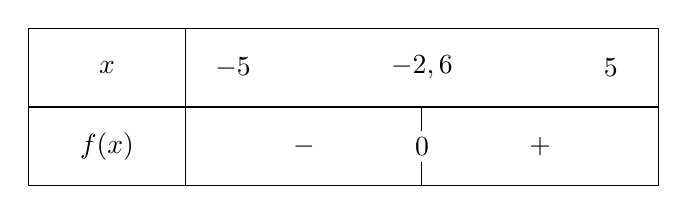
\begin{tikzpicture}
			\draw (0,0) -- ++(8,0) -- ++(0,-2) -- ++(-8,0) -- cycle;
			\draw (0,-1) -- ++(8,0);
			\draw (2,0) -- ++(0,-2);

			\node at (1,-0.5) {$x$};
			\node at (2.6,-0.5) {$-5$};
			\node at (5,-0.5) {$-2,6$};
			\node at (7.4,-0.5) {$5$};

			\node at (1,-1.5) {$f(x)$};
			\node at (3.5,-1.5) {$-$};
			\node at (5,-1.5) {$0$};
			\node at (6.5,-1.5) {$+$};
			\draw (5,-1) -- ++(0,-0.3) ++ (0,-0.4) -- ++(0,-0.3);
		\end{tikzpicture}
	\end{center}

	Le tableau de variations de $f$ est :

	\begin{center}
		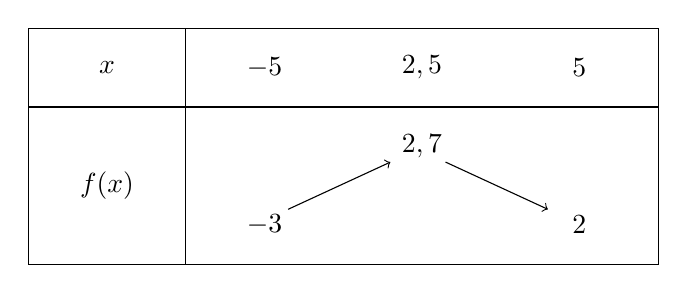
\begin{tikzpicture}
			\draw (0,0) -- ++(8,0) -- ++(0,-3) -- ++(-8,0) -- cycle;
			\draw (0,-1) -- ++(8,0);
			\draw (2,0) -- ++(0,-3);

			\node at (1,-0.5) {$x$};
			\node at (3,-0.5) {$-5$};
			\node at (5,-0.5) {$2,5$};
			\node at (7,-0.5) {$5$};

			\node at (1,-2) {$f(x)$};
			\node at (3,-2.5) {$-3$};
			\node at (5,-1.5) {$2,7$};
			\node at (7,-2.5) {$2$};

			\draw[->] (3.3,-2.3) -- (4.6,-1.7);
			\draw[->] (5.3,-1.7) -- (6.6,-2.3);
		\end{tikzpicture}
	\end{center}
\end{exemple}

\section{Fonction affine}

\begin{definition}[Fonction affine]
	Une \textbf{fonction affine} est une fonction telle que $f(x) = ax + b$, avec $a$ et $b$ deux nombres réels.
\end{definition}

\begin{propriete}[Graphe d'une fonction affine]
	Le graphe d'un fonction affine est une \textbf{droite}, telle que :
	\begin{itemize}
		\item La pente de cette droite est $a$.
		\item La droite passe par le point $(0 ; b)$.
	\end{itemize}
\end{propriete}

\begin{exemple}
	La fonction $f(x) = 2x$ a pour graphe
	\begin{center}
		\begin{tikzpicture}
			\draw[thin,gray] (-4.5,-4.5) grid (4.5,4.5);
			\draw[thick,\myArrow] (-4.5,0) -- (4.5,0);
			\draw[thick,\myArrow] (0,-4.5) -- (0,4.5);
			\draw (1,0) -- ++(0,-0.2) node[below] {$1$};
			\draw (0,1) -- ++(-0.2,0) node[left] {$1$};

			\draw[orange,ultra thick,variable=\x,domain=-2.25:2.25] plot({\x},{2*\x}) node[right] {$𝒞_f$};
		\end{tikzpicture}
	\end{center}

	La fonction $g(x) = -\dfrac{x}{2} + 1$ a pour graphe
	\begin{center}
		\begin{tikzpicture}
			\draw[thin,gray] (-4.5,-4.5) grid (4.5,4.5);
			\draw[thick,\myArrow] (-4.5,0) -- (4.5,0);
			\draw[thick,\myArrow] (0,-4.5) -- (0,4.5);
			\draw (1,0) -- ++(0,-0.2) node[below] {$1$};
			\draw (0,1) -- ++(-0.2,0) node[left] {$1$};

			\draw[orange,ultra thick,variable=\x,domain=-4.5:4.5] plot({\x},{-\x/2 + 1}) node[right] {$𝒞_g$};
		\end{tikzpicture}
	\end{center}
\end{exemple}

\end{document}